\documentclass[11pt]{exam}
\RequirePackage{amssymb, amsfonts, amsmath, latexsym, verbatim, xspace, setspace}
\RequirePackage{tikz, pgflibraryplotmarks,pgfplots}

\usepackage[margin=1in]{geometry}

\newcommand{\class}{AP Calculus AB}
\newcommand{\term}{2016-2017}
\newcommand{\examnum}{Problem Set 2}
\newcommand{\examdate}{2016-17}
\newcommand{\timelimit}{40 Minutes (Suggested)}
\singlespacing
\parindent 0ex
\begin{document} 
	\pagestyle{head}
	\firstpageheader{}{}{}
	\runningheader{\class}{\examnum\ - Page \thepage\ of \numpages}{\examdate}
	\runningheadrule
	
	\begin{flushright}
		\begin{tabular}{p{2.8in} r l}
			\textbf{\class} & \textbf{Name (Print):} & \makebox[2in]{\hrulefill}\\
			\textbf{\term} &&\\
			\textbf{\examnum} &&\\
			\textbf{Time Limit: \timelimit}
		\end{tabular}\\
	\end{flushright}
	\rule[1ex]{\textwidth}{.1pt}
	This set contains \numpages\ pages (including this cover) and \numquestions\ problems. These problems correspond to the topics taught in \textsection 2: Derivatives. The problems included here are similar to those that will be asked on the AP Test. All answers should be completed to the best of your ability with \textit{all} work shown.
	\newpage
	\begin{questions}
		\addpoints
		\question[15] The derivative shown gives the slope of a function for any generic $x$ for some generic function $f(x)$. Write the simplest limit to find the derivative of a generic function $f(x)$ at a specific point $x=c$. Hint: when $x=c$, $f(x)=f(c)$.
		
		% Question with parts
		\newpage
		\addpoints
		\question[5] Estimate the derivative at $x=0$ and $x=1$
		\begin{center}
			\begin{tikzpicture}
				\begin{axis}[axis lines=center]
				\addplot[blue,domain=-2:2]{(x-1)*(x+1)*(x+2)};
				\end{axis}
			\end{tikzpicture}
		\end{center}
		\newpage\addpoints
		\question[15] Calculate the derivative:
		\noaddpoints 
		\begin{parts}
			\part[5] $f(x)=\ln(x^2)$
			\vspace{2.5in}
			\part[5] $g(x)=\sin(x)*e^{2x}$.
			\vspace{2.5in}
			\part[5] $\displaystyle\frac{5\sqrt{x}}{x^3+5x^2-1}$
		\end{parts}
		\newpage\addpoints
		\question[10] Find the derivative of $(x-3)^2+(y-2)^2=9$ using implicit differentiation
		\newpage\addpoints
		\question[20] Find the local maximums and minimums of $f(x)=x^3+1.5x^2-6x+5$ on the inverval [-5,2]. Also, find the intervals where $f(x)$ is concave up and concave down.
		\newpage\addpoints
		\question[10] Graph the derivative of the function given on the blank graph below:
		\begin{center}
		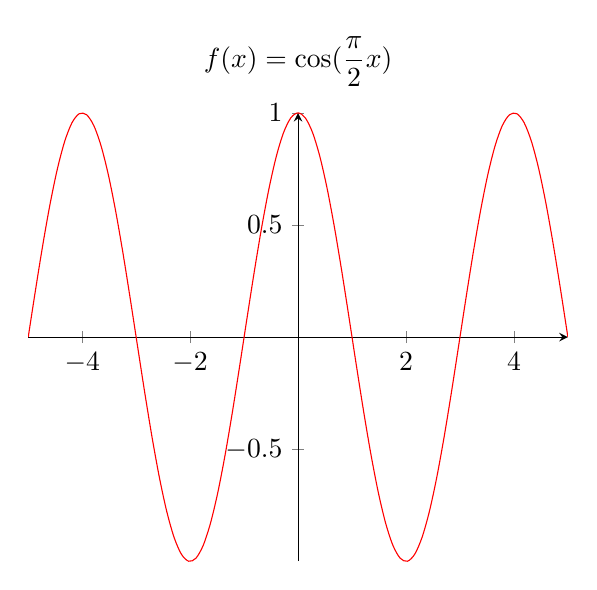
\begin{tikzpicture}
			\begin{axis}[axis lines=middle,title={$f(x)=\cos(\displaystyle\frac{\pi}{2} x)$}]
			\addplot[red,domain=-5:5,samples=75,smooth]{cos(90*x)};
			\end{axis}
		\end{tikzpicture}
	\end{center}
		\vspace{1in}
		\begin{center}
		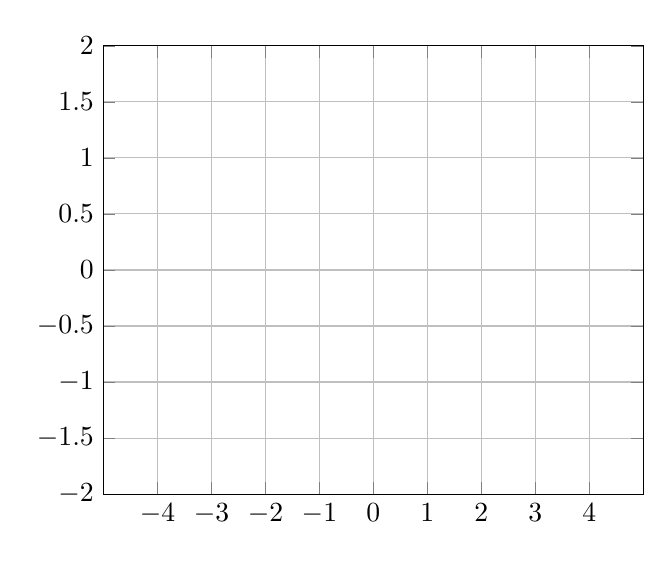
\begin{tikzpicture}
			\begin{axis}[grid,ymin=-2,ymax=2,ytick={-2,-1.5,...,2},xmin=-5,xmax=5,xtick={-4,...,4}]
			\addplot[draw=none] coordinates {(0,0)};
			\end{axis}
		\end{tikzpicture}
	\end{center}
		\newpage\addpoints
		\question[10] Is the function \[
		f(x)=
		\begin{cases}
		-x & x\leq -1\\
		x^3+2x^2 & x>1 
		\end{cases}
		\]
		differentiable everywhere?
	\end{questions}
\end{document}